\documentclass[12pt]{article}
\usepackage[letterpaper, margin=1in, headheight=105pt]{geometry}
\usepackage{graphicx}
\usepackage{amsmath}
\usepackage{xcolor}
\usepackage{minted}
\usepackage{comment}
\usemintedstyle{manni}
\pagestyle{empty}

\begin{document}
\begin{comment}
\setcounter{section}{1}
\section{Homework Coding Part}
\setcounter{subsection}{1}
\subsection{Bayesian Spam Filtering}
The test error for Bayesian classifier is 11.00\%, while the majority class predictor has test error 38.56\%.
So we con conclude that the Bayesian classifier is working.
\inputminted[frame=single,framesep=10pt,linenos,xleftmargin=\parindent]{octave}{./hw2/problem2/Bayesian_spam_filtering.m}
\setcounter{subsection}{3}
\subsection{Handwritten digit classification with logistic regression}
The test error is 5.40\%.
My termination criterion is
\[ \frac{||\theta_{t+1}-\theta_{t}||}{||\theta_t||}<0.001 \]
The value of the objective function at the optimum is \(6381.5\).
Since the logistic regression rely on \(\eta(x)\) which is a probability, we take the difference between these probabilities and the threshold \(\frac{1}{2}\), and take the absolute value.
\[ \left|\eta(x)-\frac{1}{2}\right| \]
The larger this value is, the more confident the regression classifier is about its prediction.
\inputminted[frame=single,framesep=10pt,linenos,xleftmargin=\parindent]{octave}{./hw2/problem4/Handwritten_digit_classification.m}
\begin{figure}
    \centering
    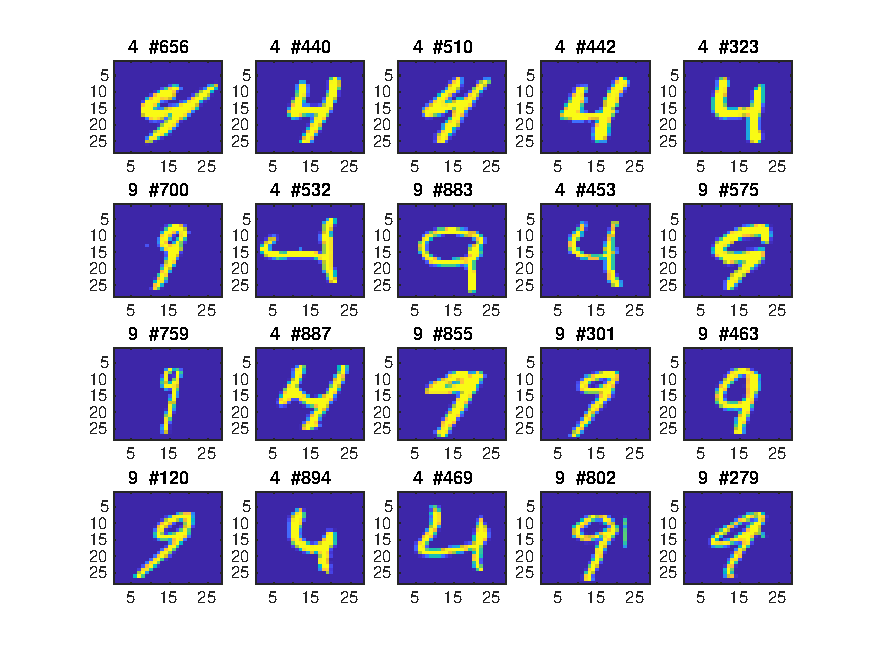
\includegraphics[width=0.85\textwidth]{./hw2/problem4/hw2p4b.pdf}
    \caption{Top 20 mis-classified images}
\end{figure}
\end{comment}

\setcounter{section}{2}
\section{Homework Coding Part}
\subsection{Linear Regression}
\inputminted[frame=single,framesep=10pt,linenos,xleftmargin=\parindent]{octave}{./hw3/problem1/Linear_regression.m}
The mean square error for ordinary linear regression is \(22.2826\).
The mean square error for regularized least squares regression is \(21.4859\).
The predicted response at the input \(x=[100, 100]\) is \(24.4581\).
The regularized least squares regression (Ridge) has parameter
\[ w=[ 0.6487, -0.0632]^T \hspace{2em} b=-34.0834 \]
\subsection{Robust Regression}
\paragraph{(a)}
In order to be consistent with the higher dimension case, I denote \(\theta=[b, w]^T\), \(\tilde{x}_i=[1; x_i]\).
The majoring function is
\[ \bar{J} (\theta;\theta_t)=\sum_{i=1}^{n}\left[\rho(y_i-\tilde{x}_i^T\theta_t)-\frac{y_i-\tilde{x}_i^T\theta_t}{2}\rho'(y_i-\tilde{x}_i^T\theta_t) \right]+\frac{1}{2}\sum_{i=1}^{n}\frac{\rho'(y_i-\tilde{x}_i^T\theta_t)}{y_i-\tilde{x}_i^T\theta_t}\left(y_i-\tilde{x}_i^T\theta\right) \]
The first sum doesn't contain \(\theta\), so it has nothing to do with mininizing.
The second sum is exactly the reweighted least squares, as it can be written as
\[ \frac{1}{2}(y-\tilde{x}^T\theta)^T C (y-\tilde{x}^T\theta) \hspace{1em}\textrm{where } C=\texttt{diag}\left(\frac{\rho'(y_i-\tilde{x}_i^T\theta_t)}{y_i-\tilde{x}_i^T\theta_t}\right) \]
Thus, the iteration becomes
\[ \theta_{t+1}=\left(\tilde{x}^TC\tilde{x}\right)^{-1}\tilde{x}^TCy \]
Hence, the majoring-mininizing algorithm can be understood as ``iteratively reweighted least squares''.
It achieves robustness by assigning \emph{lower} weights for outliers and \emph{higher} weights for inliers, since by lemma, the weight function \(\frac{\rho'(r)}{r}\) is a non-increasing function on \(r\).
\paragraph{(b)}
As we can see, by picking specific \(\rho\) with \(\rho(r)=\sqrt{1+r^2}+1\), we have its derivative
\[ \rho'(r)=\frac{r}{\sqrt{1+r^2}} \]
Then, the weights for this specific \(\rho\) are
\[ \frac{\rho'(r_{t,i})}{r_{t_i}}=\frac{1}{\sqrt{1+r_{t,i}^2}}=\frac{1}{\sqrt{1+\left(y_i-\tilde{x}_i^T\theta_t\right)^2}} \]
The parameters from MM algorithm and ordinary linear regression are
\begin{center}
\begin{tabular}{c|cc}
    & \(w\) & \(b\) \\ \hline
    robust & \(7.4933\) & \(6.2352\) \\ \hline
    ordinary & \(-0.8061\) & \(10.5285\)
\end{tabular}
\end{center}
\begin{figure}[htbp]
    \centering
    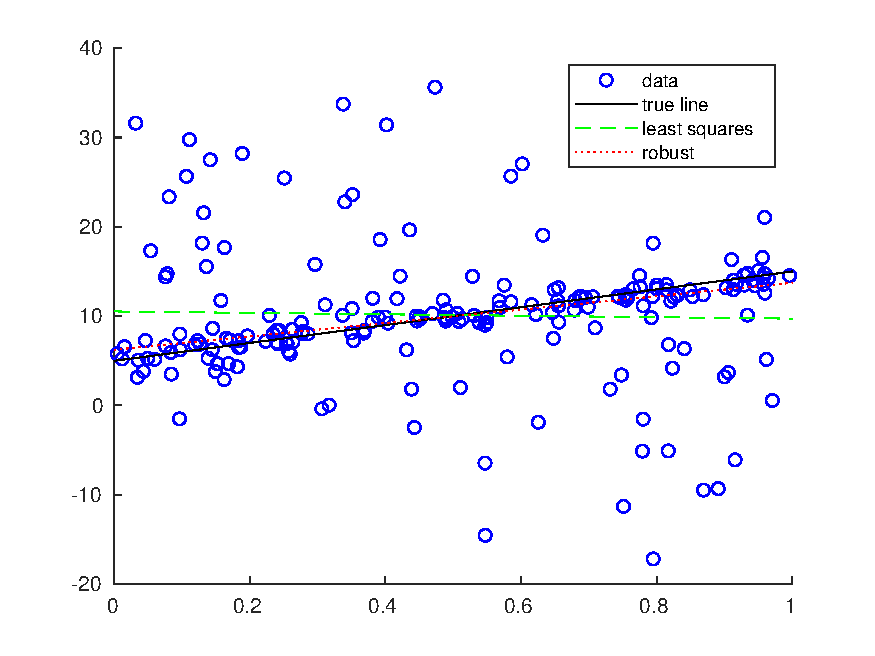
\includegraphics[width=0.85\textwidth]{./hw3/problem2/hw3p2.pdf}
    \caption{Data, true line, OLS estimate, robust estimate}
\end{figure}
\inputminted[frame=single,framesep=10pt,linenos,xleftmargin=\parindent]{octave}{./hw3/problem2/Robust_regression.m}
\setcounter{subsection}{3}
\subsection{Subgradient methods for the optimal soft margin hyperplane}
\paragraph{(a)}
We pick \(J_i(w,b)\) to be
\[ J_i(w,b)=\frac{1}{n}L(y_i,w^T x_i+b)+\frac{\lambda}{2n} w^T w \]
This gives
\[ J(w,b)=\sum_{i=1}^{n}J_i(w,b)=\frac{1}{n}\sum_{i=1}^{n}\left[L(y_i,w^T x_i+b) \right] +\frac{\lambda}{2}w^T w \]
To choose a subgradient for the non-differentiable function, we take
\[ \frac{\partial L(y,t)}{\partial t}=\frac{1}{2}\left[\mathtt{sign}(t-y)-y \right] \]
which provides
\[ \frac{\partial L(y,t)}{\partial t}=\begin{cases} [\mathtt{sign}(t-1)-1]/2 & y=1 \\ [\mathtt{sign}(t+1)+1]/2 & y=-1 \end{cases} \]
By chain rule,
\begin{align*}
    \frac{\partial{J_i(w,b)}}{\partial b}&=\frac{1}{2n}[\mathtt{sign}(w^T x_i+b-y_i)-y_i] \\
    \nabla_w J_i(w,b)&=\frac{x_i}{2n}[\mathtt{sign}(w^T x_i+b-y_i)-y_i]+\frac{\lambda}{n}w
\end{align*}
As usual trick, denote  \(\theta=[b, w]^T\), \(\tilde{x}_i=[1; x_i]\).
Then, the subgradient with respect to \(\theta\) is the concatenated vector of the previous two.
\[ u_i= \nabla J_i(\theta)=\begin{bmatrix}[\mathtt{sign}(w^T x_i+b-y_i)-y_i]/2n \\ x_i[\mathtt{sign}(w^T x_i+b-y_i)-y_i]/2n+\lambda w/n \end{bmatrix} \]
\paragraph{(b)}
The estimated hyperplane parameters are
\[ w=\begin{bmatrix} -2.8921 \\ 14.3929 \end{bmatrix} \hspace{2em} b=-0.9761 \]
The minimum achieved value of the objective function is
\[ J(w,b)=0.3012 \]
The two figures are shown in Figure \ref{hw3p4b}.
\begin{figure}[htbp]
    \centering
    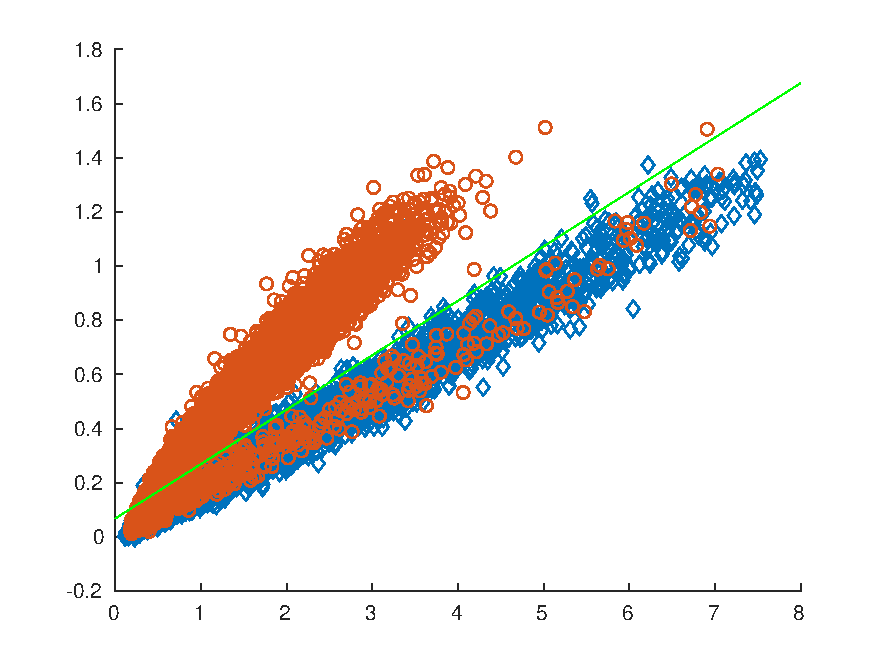
\includegraphics[width=0.85\textwidth]{./hw3/problem4/hw3p4b1.pdf}
    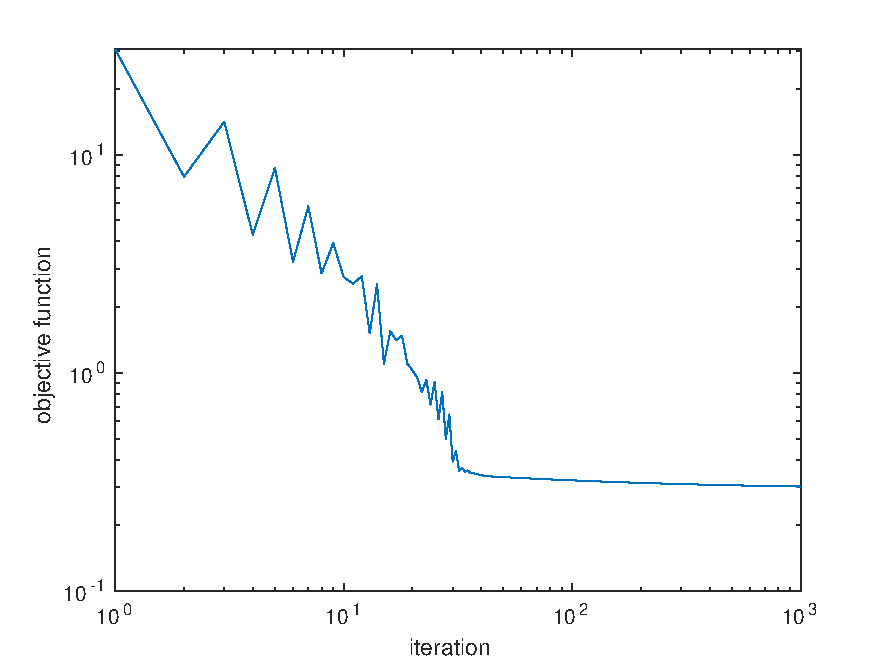
\includegraphics[width=0.85\textwidth]{./hw3/problem4/hw3p4b2.pdf}
    \caption{Subgradient Learned separating hyperplane and Loss by iteration}
    \label{hw3p4b}
\end{figure}
\paragraph{(c)}
The estimated hyperplane parameters are
\[ w=\begin{bmatrix} -5.9996 \\ 25.6366 \end{bmatrix} \hspace{2em} b=-2.3141 \]
The minimum achieved value of the objective function is
\[ J(w,b)=0.2935 \]
The two figures are shown in Figure \ref{hw3p4c}.
\begin{figure}[htbp]
    \centering
    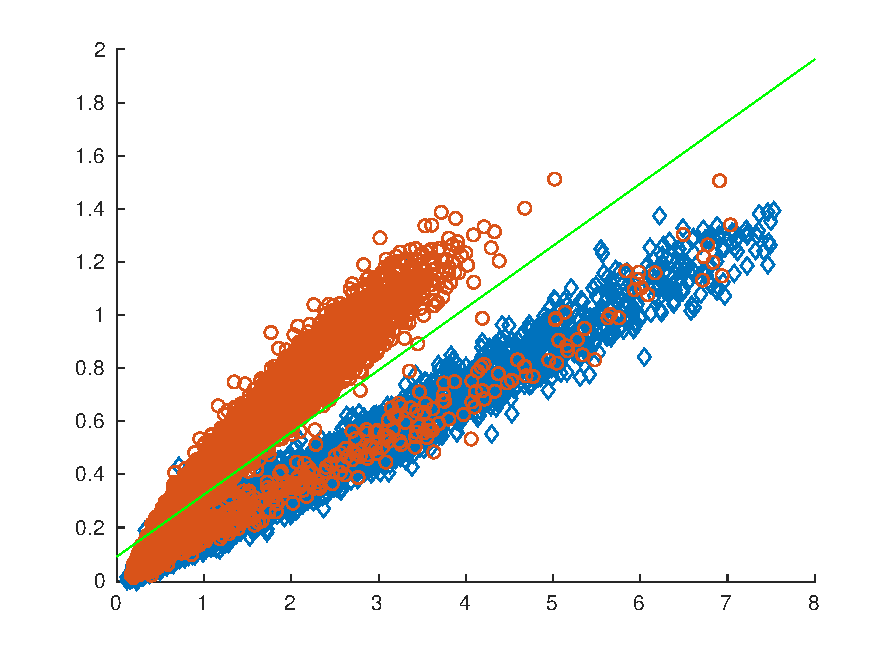
\includegraphics[width=0.85\textwidth]{./hw3/problem4/hw3p4c1.pdf}
    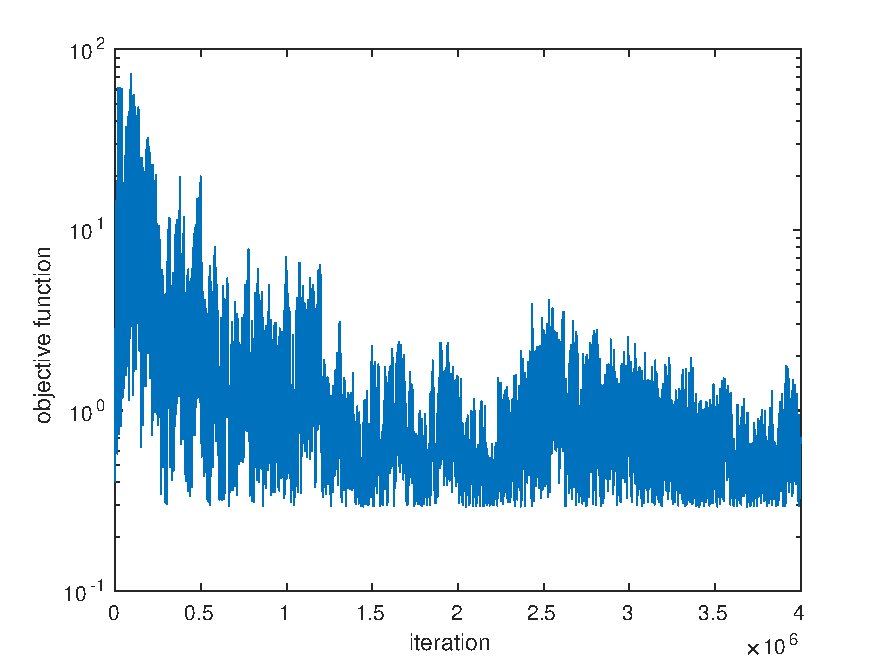
\includegraphics[width=0.85\textwidth]{./hw3/problem4/hw3p4c2.pdf}
    \caption{Stochastic subgradient Learned separating hyperplane and Loss by iteration}
    \label{hw3p4c}
\end{figure}
\paragraph{(d)}
The subgradient method is more stable, but the optimizer obtained by the subgradient method may not be as optimal as the stochastic subgradient method.
This is because stochastic subgradient method updates much more frerquently than the subgradient method, so it has better chance to hit a lower objective function.
However, we can see that there is no sign of convergence for stochastic subgradient method at the end of iteration, although it is indeed much better than the initial period (the \(y\)-axis is in log scale).
By contrast, the subgradient method converges quite well at the end of iteration, as we can see the curve is nearly flat.
\paragraph{(e)}
\inputminted[frame=single,framesep=10pt,linenos,xleftmargin=\parindent]{octave}{./hw3/problem4/subgradient.m}
\inputminted[frame=single,framesep=10pt,linenos,xleftmargin=\parindent]{octave}{./hw3/problem4/stochastic.m}
\end{document}